\documentclass[conference]{IEEEtran}
\IEEEoverridecommandlockouts

\usepackage[utf8]{inputenc}
\usepackage[T5]{fontenc}
\usepackage[vietnamese]{babel}
\usepackage{cite}
\usepackage{amsmath,amssymb,amsfonts}
\usepackage{graphicx}
\usepackage{textcomp}
\usepackage{xcolor}
\usepackage{booktabs}
\usepackage{multirow}
\usepackage{url}
\usepackage{hyperref}
\usepackage{float}
\usepackage{listings}
\usepackage{enumitem}

% Cấu hình hyperlink
\hypersetup{
    colorlinks=true,
    linkcolor=blue!70!black,
    citecolor=green!50!black,
    urlcolor=blue!80!black,
}

% Cấu hình code listing
\lstset{
    language=Python,
    basicstyle=\ttfamily\small,
    keywordstyle=\color{blue},
    stringstyle=\color{red},
    commentstyle=\color{green!60!black},
    backgroundcolor=\color{gray!10},
    showspaces=false,
    showstringspaces=false,
    frame=single,
    tabsize=2,
    breaklines=true,
    breakatwhitespace=false,
    captionpos=b,
    aboveskip=1.5em,
    belowskip=1.5em
}

\begin{document}

% ======================== TRANG BÌA ========================
\begin{titlepage}
\begin{center}

\vspace*{0.5cm}

{\large\bfseries BỘ GIÁO DỤC VÀ ĐÀO TẠO}\\[0.2cm]
{\large\bfseries TRƯỜNG ĐẠI HỌC ĐẠI NAM}\\[0.3cm]
{\large Khoa Công nghệ Thông tin}

\vspace{1.5cm}

\rule{\linewidth}{0.5pt}\\[0.4cm]
{\LARGE\bfseries NHẬN DẠNG CỬ CHỈ TAY\\[0.3cm]
ĐIỀU KHIỂN THIẾT BỊ HỖ TRỢ\\[0.3cm]
CHĂM SÓC BỆNH NHÂN\\[0.3cm]
TRONG PHÒNG BỆNH THÔNG MINH}\\[0.4cm]
\rule{\linewidth}{0.5pt}

\vspace{1cm}

{\large\bfseries Môn học: Trí tuệ nhân tạo}

\vspace{1cm}

{\large
\begin{tabular}{ll}
\textbf{Nhóm thực hiện:} & Nhóm 11 \\
\textbf{Thành viên:} & Lã Anh Tuấn (Nhóm trưởng) \\
 & Kiều Đức Anh \\
 & Dương Duy Khánh \\
\textbf{Giảng viên hướng dẫn:} & TS. Lê Trung Hiếu \\
\end{tabular}
}

\vspace{1cm}

{\large Hà Nội, 2026}

\end{center}
\end{titlepage}

% ======================== NỘI DUNG CHÍNH ========================
\title{Nhận dạng cử chỉ tay điều khiển thiết bị\\hỗ trợ chăm sóc bệnh nhân\\trong phòng bệnh thông minh}

\author{
\IEEEauthorblockN{Lã Anh Tuấn, Kiều Đức Anh, Dương Duy Khánh}
\IEEEauthorblockA{Nhóm 11 --- Khoa Công nghệ Thông tin\\
Trường Đại học Đại Nam, Hà Nội, Việt Nam\\
GVHD: TS. Lê Trung Hiếu}
}

\maketitle

% ======================== TÓM TẮT ========================
\begin{abstract}
Trong môi trường y tế hiện đại, việc hỗ trợ bệnh nhân tương tác với các thiết bị trong phòng bệnh mà không cần tiếp xúc vật lý là nhu cầu cấp thiết. Bài báo trình bày hệ thống nhận dạng cử chỉ tay thời gian thực sử dụng mô hình YOLOv8 Nano (Custom) để điều khiển thiết bị hỗ trợ chăm sóc bệnh nhân trong phòng bệnh thông minh. Hệ thống nhận dạng 6 cử chỉ tay: \textbf{Nắm tay} (bật/tắt đèn), \textbf{Chỉ ngón trỏ} (nâng/hạ giường), \textbf{Xòe tay} (SOS khẩn cấp), \textbf{Vuốt trái/phải} (kéo/mở rèm) và \textbf{Vẫy tay} (gọi bác sĩ). Bộ dữ liệu gồm \textbf{2.561 ảnh} (Tập huấn luyện: 2.049 ảnh, Tập Val: 512 ảnh) được gán nhãn và huấn luyện trên Google Colab với GPU Tesla T4. Mô hình đạt mAP@0.5 = \textbf{97,1\%}. Hệ thống tích hợp bộ lọc Dwell-time 5 giây chống kích hoạt nhầm, phản hồi bằng giọng nói tiếng Việt (TTS) và giao diện Dashboard web hoạt động 100\% offline.
\end{abstract}

\begin{IEEEkeywords}
nhận dạng cử chỉ tay, YOLOv8, phòng bệnh thông minh, điều khiển không tiếp xúc, học sâu, IoT y tế, Text-to-Speech
\end{IEEEkeywords}

% ======================== 1. ĐẶT VẤN ĐỀ ========================
\section{Đặt vấn đề}

Trong môi trường y tế hiện đại, đặc biệt tại các phòng bệnh hồi sức tích cực hoặc phòng chăm sóc bệnh nhân đặc biệt, khả năng tương tác của bệnh nhân với môi trường xung quanh gặp nhiều hạn chế nghiêm trọng. Việc sử dụng nút bấm vật lý truyền thống gặp các trở ngại:

\begin{itemize}[noitemsep]
    \item Khó tiếp cận đối với bệnh nhân bị hạn chế vận động.
    \item Nguy cơ lây nhiễm chéo vi khuẩn/virus qua bề mặt tiếp xúc.
    \item Không tiện dụng trong các tình huống khẩn cấp.
    \item Phụ thuộc vào nhân viên y tế cho các thao tác đơn giản.
\end{itemize}

Giao tiếp bằng cử chỉ tay là phương thức tự nhiên và trực quan cho con người. Nhiều nghiên cứu đã chứng minh tính khả thi của nhận dạng cử chỉ tay bằng thị giác máy tính \cite{ref1}. Tuy nhiên, hầu hết hệ thống hiện có chưa đáp ứng đặc thù môi trường y tế --- nơi đòi hỏi \textbf{độ tin cậy cao}, \textbf{phản hồi thời gian thực} và \textbf{cơ chế an toàn chống kích hoạt nhầm}.

Dự án đề xuất xây dựng hệ thống \textbf{Smart Hospital Room} --- hỗ trợ bệnh nhân điều khiển thiết bị phòng bệnh thông qua 6 cử chỉ tay không tiếp xúc, sử dụng mô hình YOLOv8 Nano \cite{ref7} kết hợp bộ lọc an toàn Dwell-time và phản hồi giọng nói tiếng Việt.

\textbf{Ba đóng góp chính:}
\begin{enumerate}[noitemsep]
    \item Xây dựng bộ dữ liệu cử chỉ tay chuyên biệt gồm 2.561 ảnh với \textbf{3 lớp nhận dạng} (Nam\_Tay, Chi\_Ngon\_Tro, Xoe\_Tay). Cử chỉ động (Vuốt, Vẫy) được suy diễn từ quỹ đạo chuyển động của lớp Xoe\_Tay thông qua module MotionTracker, không cần class riêng.
    \item Thiết kế kiến trúc nhận dạng thời gian thực với bộ lọc Anti-flicker + Dwell-time 5 giây đảm bảo an toàn y tế.
    \item Triển khai ứng dụng web hoàn chỉnh với Dashboard điều khiển, giọng nói TTS tiếng Việt, hoạt động 100\% offline.
\end{enumerate}

% ======================== 2. NGHIÊN CỨU LIÊN QUAN ========================
\section{Các nghiên cứu liên quan}

\subsection{Phương pháp dựa trên đặc trưng thủ công}
Các nghiên cứu ban đầu sử dụng MediaPipe Hands để trích xuất 21 điểm mốc (landmarks) trên bàn tay, sau đó áp dụng các bộ phân loại truyền thống như Random Forest, KNN hoặc SVM \cite{ref1}. Phương pháp này nhẹ nhưng phụ thuộc vào chất lượng phát hiện landmark và không có khả năng định vị vùng tay trong ảnh.

\subsection{Phương pháp dựa trên học sâu}
Các mô hình CNN như ResNet \cite{ref9}, EfficientNet và Vision Transformer (ViT) \cite{ref5} đạt hiệu năng cao trong phân loại cử chỉ. Tuy nhiên, các mô hình phân loại thuần túy không cung cấp thông tin vị trí (bounding box) --- yếu tố cần thiết cho ứng dụng thời gian thực.

\subsection{Phát hiện đối tượng (Object Detection)}
Họ YOLO \cite{ref2} giải quyết đồng thời bài toán định vị và phân loại trong một lần quét, phù hợp cho ứng dụng thời gian thực. YOLOv8 \cite{ref7} là phiên bản mới nhất với kiến trúc CSPDarknet backbone, PANet neck và anchor-free detection head. Phiên bản Nano (YOLOv8n) với chỉ 3 triệu tham số cho phép triển khai trên thiết bị biên với tốc độ cao.

\begin{figure}[H]
\centering
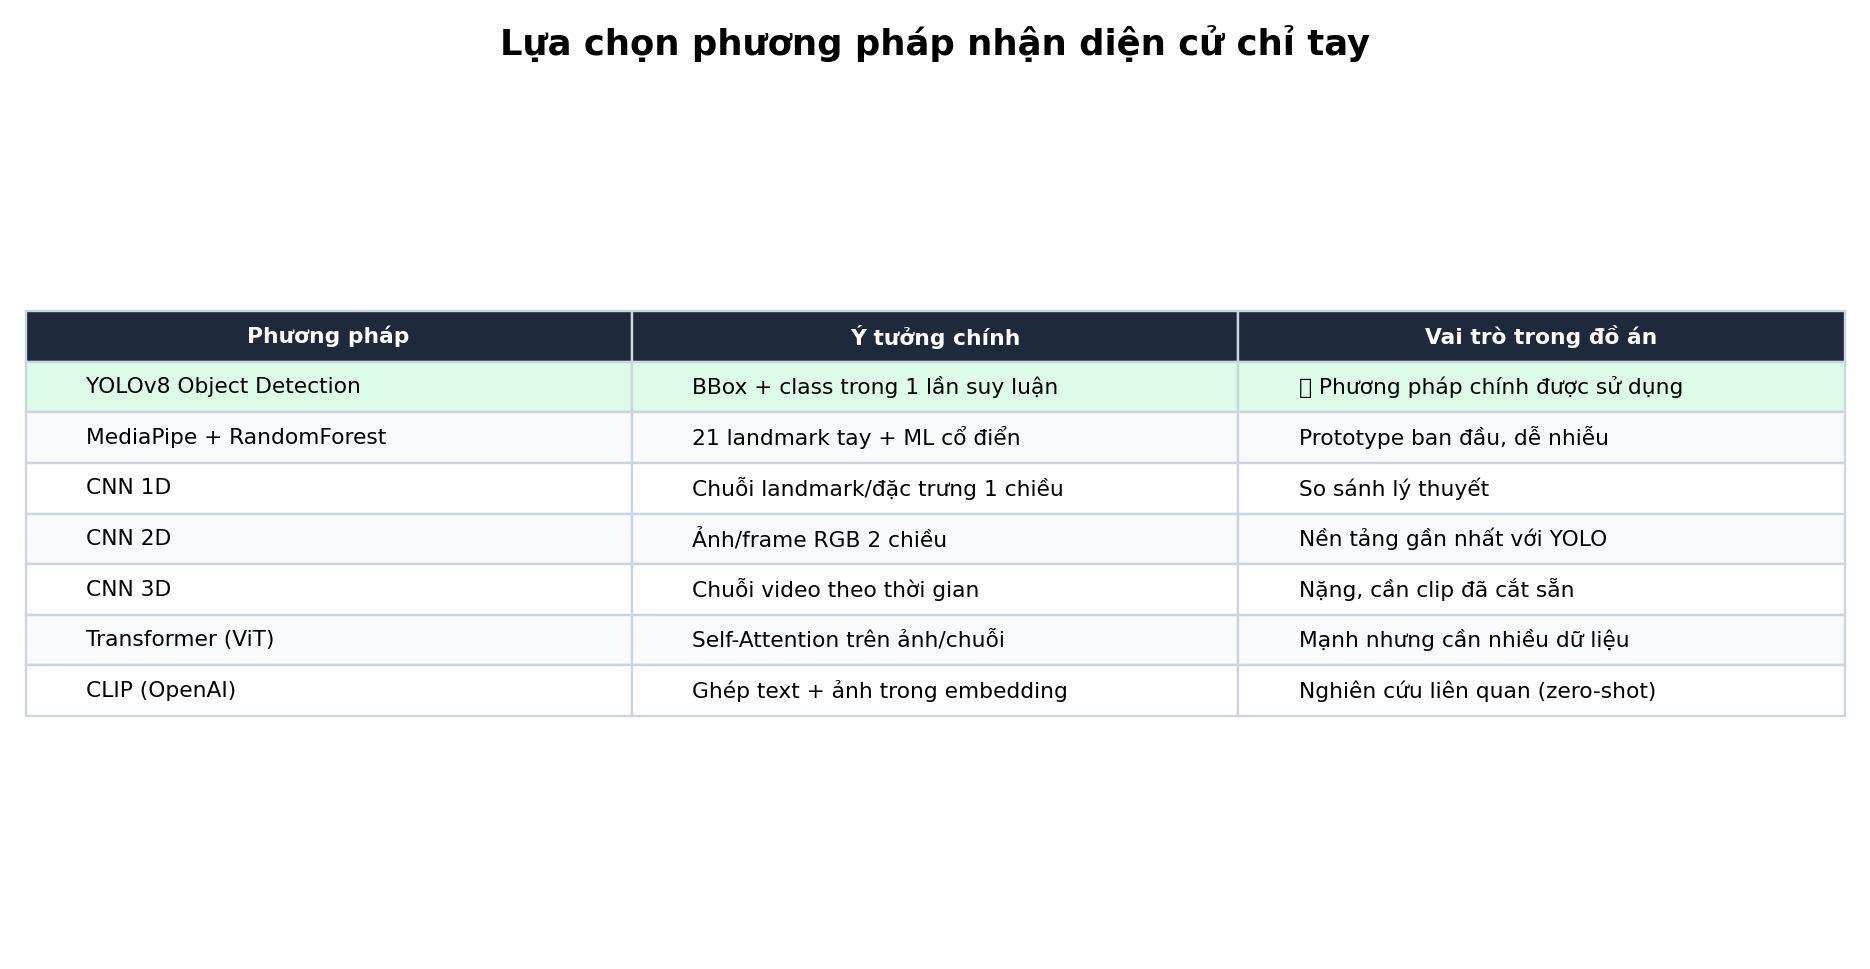
\includegraphics[width=\columnwidth]{figures/method_selection.png}
\caption{So sánh lựa chọn phương pháp nhận dạng.}
\end{figure}

\begin{figure}[H]
\centering
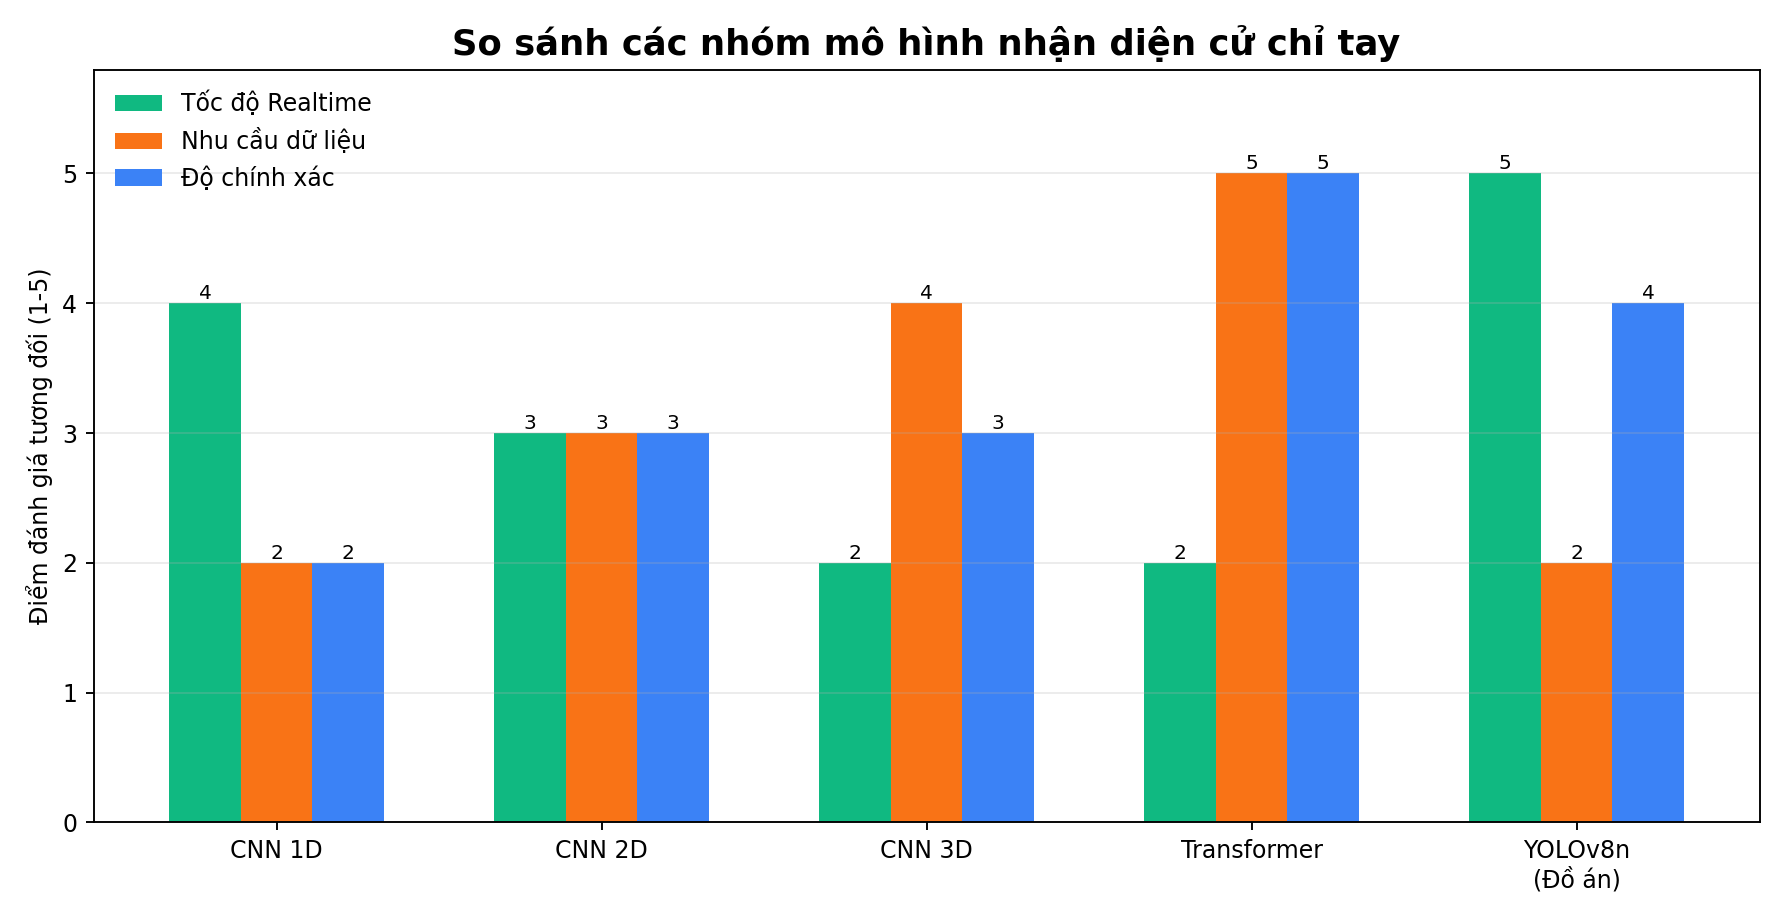
\includegraphics[width=\columnwidth]{figures/model_family_comparison.png}
\caption{So sánh các họ mô hình nhận dạng.}
\end{figure}

Trong bối cảnh phòng bệnh thông minh, một số nghiên cứu đã ứng dụng nhận dạng cử chỉ \cite{ref4}, nhưng chưa giải quyết triệt để vấn đề kích hoạt nhầm --- đặc biệt nguy hiểm trong môi trường y tế.

\begin{table}[H]
\centering
\caption{So sánh các phương pháp nhận dạng cử chỉ tay}
\label{tab:comparison}
\begin{tabular}{l|c|c|c|c}
\hline
\textbf{Phương pháp} & \textbf{Bounding Box} & \textbf{Real-time} & \textbf{Offline} & \textbf{An toàn} \\
\hline
MediaPipe + SVM & Không & Có & Có & Không \\
ResNet/EfficientNet & Không & Có & Có & Không \\
YOLOv8n (Đề xuất) & \textbf{Có} & \textbf{Có} & \textbf{Có} & \textbf{Có (Dwell-time)} \\
\hline
\end{tabular}
\end{table}

% ======================== 3. HỆ THỐNG DATASET ========================
\section{Hệ thống Dataset}

\subsection{Số lượng ảnh và Thống kê nhãn}

Bộ dữ liệu được thu thập qua nhiều đợt quay thực tế, gồm tổng cộng \textbf{2.561 ảnh} đã qua gán nhãn (annotation).
\textbf{Số lượng ảnh theo tập:}
\begin{itemize}[noitemsep]
    \item \textbf{Tập Huấn luyện (Train):} 2.049 ảnh (chiếm $\approx$80\%).
    \item \textbf{Tập Kiểm định (Val):} 512 ảnh (chiếm $\approx$20\%).
    \item Chưa tách tập Test độc lập; tập Val đóng vai trò proxy evaluation.
\end{itemize}

\textbf{Thống kê nhãn:}
\begin{figure}[H]
\centering

\includegraphics[width=\columnwidth]{figures/dataset_summary_table.png}
\caption{Bảng tổng hợp thống kê bộ dữ liệu.}
\end{figure}

\textbf{Mô tả Visualize (Matplotlib):} Các biểu đồ phân bố và trực quan hóa bộ dữ liệu (Visualize) được tạo tự động bằng thư viện Matplotlib trong hệ thống.

\begin{figure}[H]
\centering

\includegraphics[width=\columnwidth]{figures/class_distribution.png}
\caption{Phân bố số lượng ảnh theo các lớp.}
\end{figure}

\begin{figure}[H]
\centering

\includegraphics[width=\columnwidth]{figures/split_distribution.png}
\caption{Phân bố chia tách tập dữ liệu Huấn luyện và Thử nghiệm.}
\end{figure}

\subsection{Các lớp cử chỉ}

Hệ thống nhận dạng cử chỉ tay chia thành các nhóm:

\begin{figure}[h]
\centering
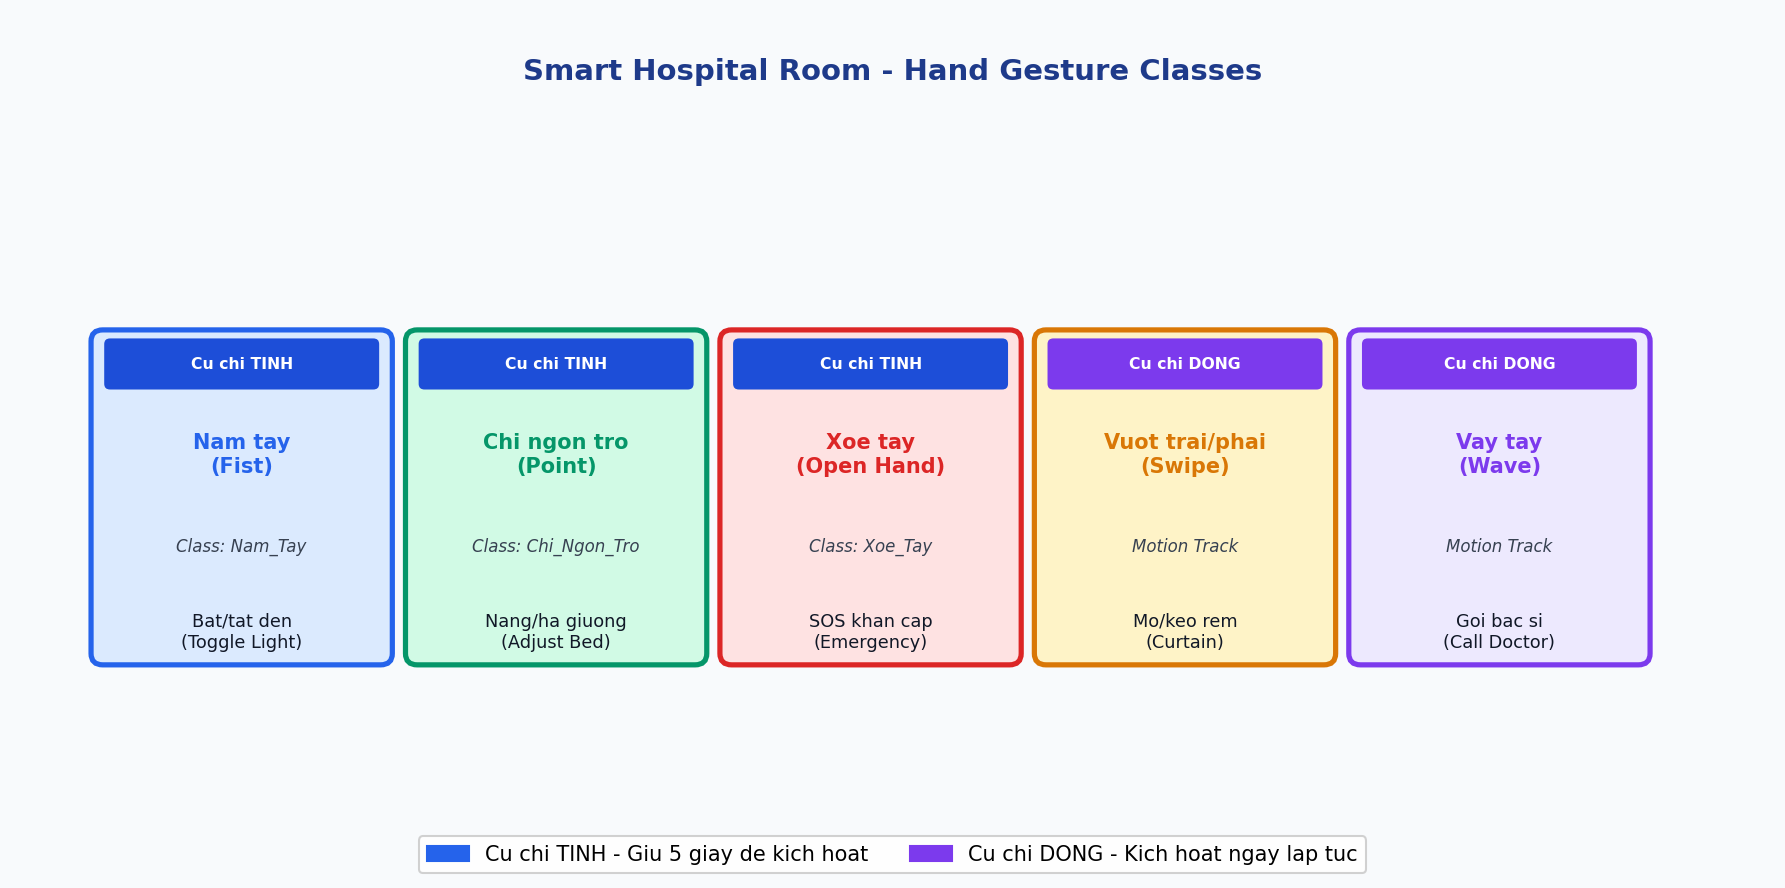
\includegraphics[width=\columnwidth]{figures/gesture_classes.png}
\caption{Các lớp cử chỉ tay và hành động tương ứng trong hệ thống.}
\label{fig:gestures}
\end{figure}

\begin{table}[h]
\centering
\caption{\textbf{Bảng I.} Định nghĩa các lớp cử chỉ và hành động}
\label{tab:classes}
\begin{tabular}{c|l|l|c}
\hline
\textbf{Loại} & \textbf{Cử chỉ} & \textbf{Hành động} & \textbf{Kích hoạt} \\
\hline
\multirow{3}{*}{Tĩnh} & Nắm tay & Bật/tắt đèn & Giữ 5s \\
 & Chỉ ngón trỏ & Nâng/hạ giường & Giữ 5s \\
 & Xòe tay & SOS khẩn cấp & Giữ 5s \\
\hline
\multirow{3}{*}{Động} & Vuốt trái & Kéo rèm vào & Tức thì \\
 & Vuốt phải & Mở rèm ra & Tức thì \\
 & Vẫy tay & Gọi bác sĩ & Tức thì \\
\hline
\end{tabular}
\end{table}

% ======================== 4. XÂY DỰNG HỆ THỐNG ========================
\section{Xây dựng Hệ thống}

\subsection{Tổng quan hệ thống}

Hệ thống được thiết kế theo mô hình luồng dữ liệu thời gian thực gồm 5 giai đoạn: (1) Thu nhận hình ảnh từ camera, (2) Nhận dạng cử chỉ qua YOLOv8, (3) Lọc chống nhiễu Anti-flicker, (4) Đếm giữ tay Dwell-time 5 giây, (5) Điều khiển thiết bị + phản hồi giọng nói.

\begin{figure}[h]
\centering
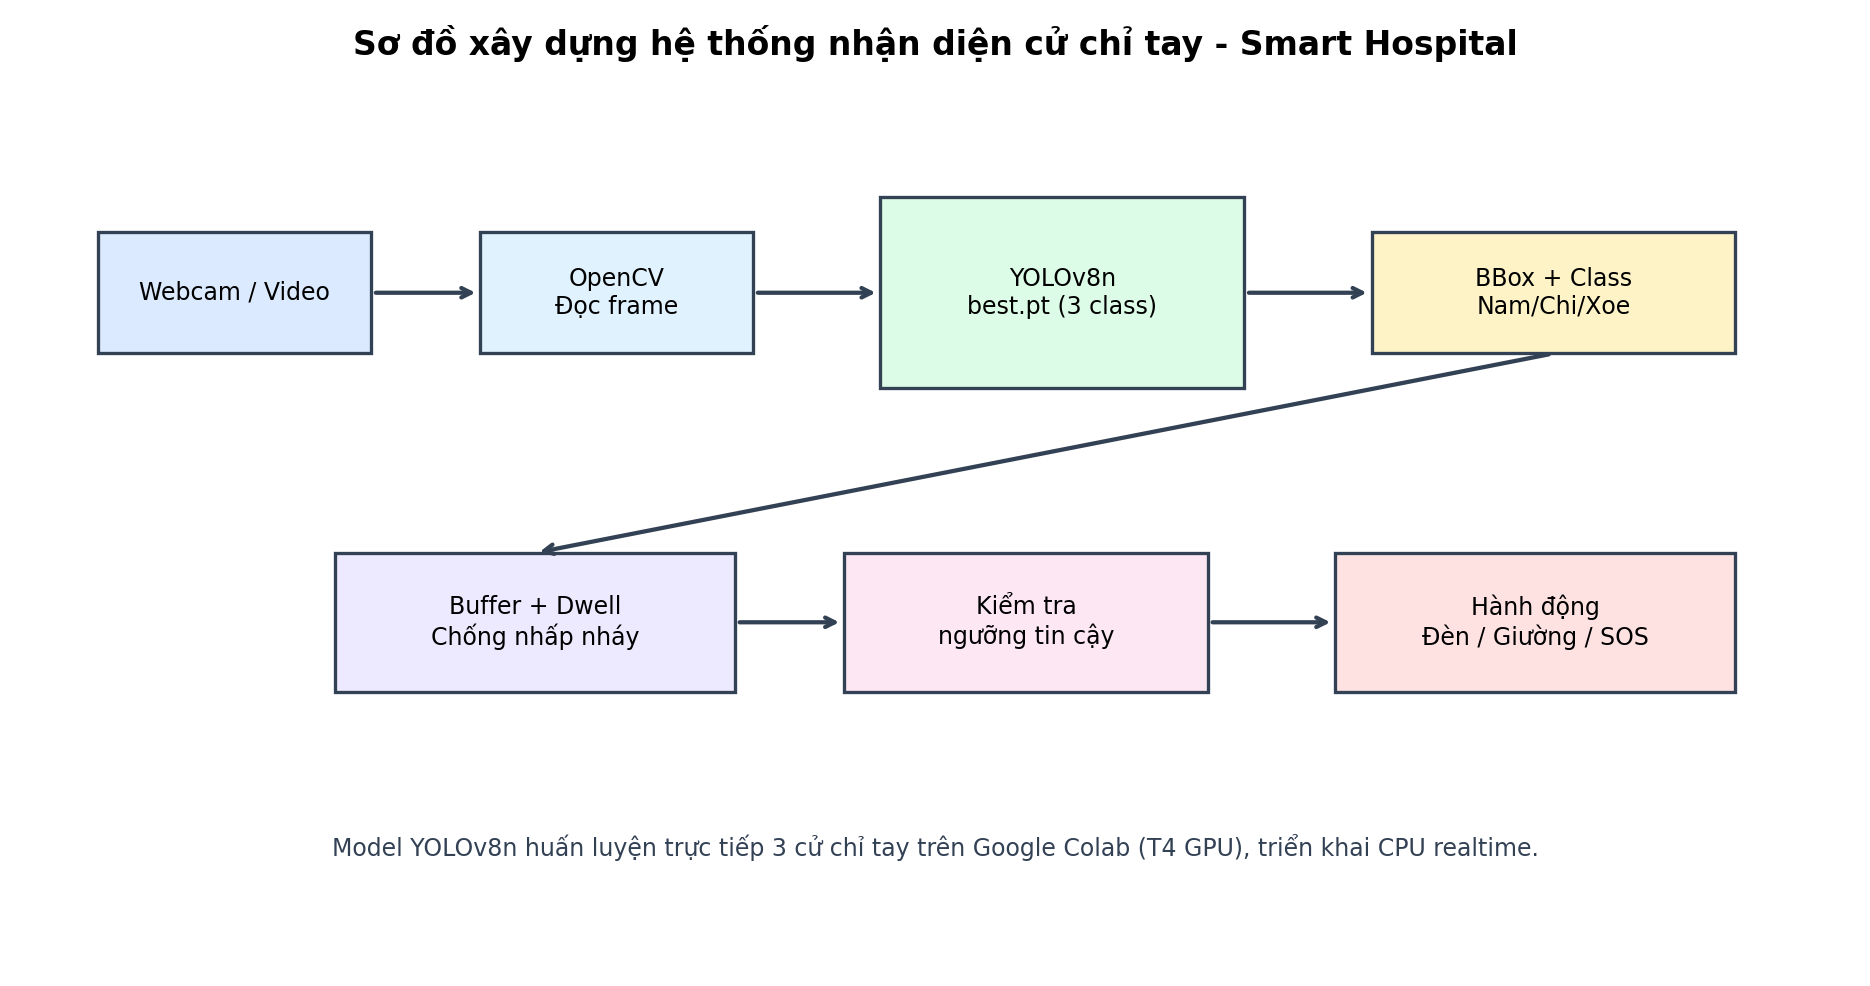
\includegraphics[width=\columnwidth]{figures/architecture_diagram.png}
\caption{Kiến trúc tổng thể hệ thống: Camera → YOLOv8 → Bộ lọc an toàn → Điều khiển thiết bị → Phản hồi giọng nói TTS.}
\label{fig:architecture}
\end{figure}

\subsection{Mô hình YOLOv8 Nano}

Kiến trúc \textbf{YOLOv8 Nano} được lựa chọn nhằm đảm bảo tốc độ phản hồi thời gian thực trên thiết bị cấu hình trung bình:

\begin{itemize}[noitemsep]
    \item \textbf{Backbone:} CSPDarknet --- giảm tham số mà giữ đặc trưng phong phú.
    \item \textbf{Neck:} PANet --- kết hợp đặc trưng đa tỉ lệ.
    \item \textbf{Head:} Anchor-free detection head --- loại bỏ anchor boxes thủ công.
    \item \textbf{Loss:} CIoU loss (regression) + BCE loss (classification).
\end{itemize}

\textbf{Trích xuất đặc trưng (Feature extraction):} Mô hình YOLOv8n (Custom) do nhóm tự huấn luyện trích xuất các đặc trưng ảnh thông qua mạng xương sống (backbone CSPDarknet). Sau đó, Detection head trả về tọa độ bounding box, nhãn class cử chỉ và độ tin cậy (confidence score). Dựa trên class này, hệ thống ánh xạ trực tiếp sang lệnh điều khiển thiết bị tương ứng.

\begin{figure}[H]
\centering
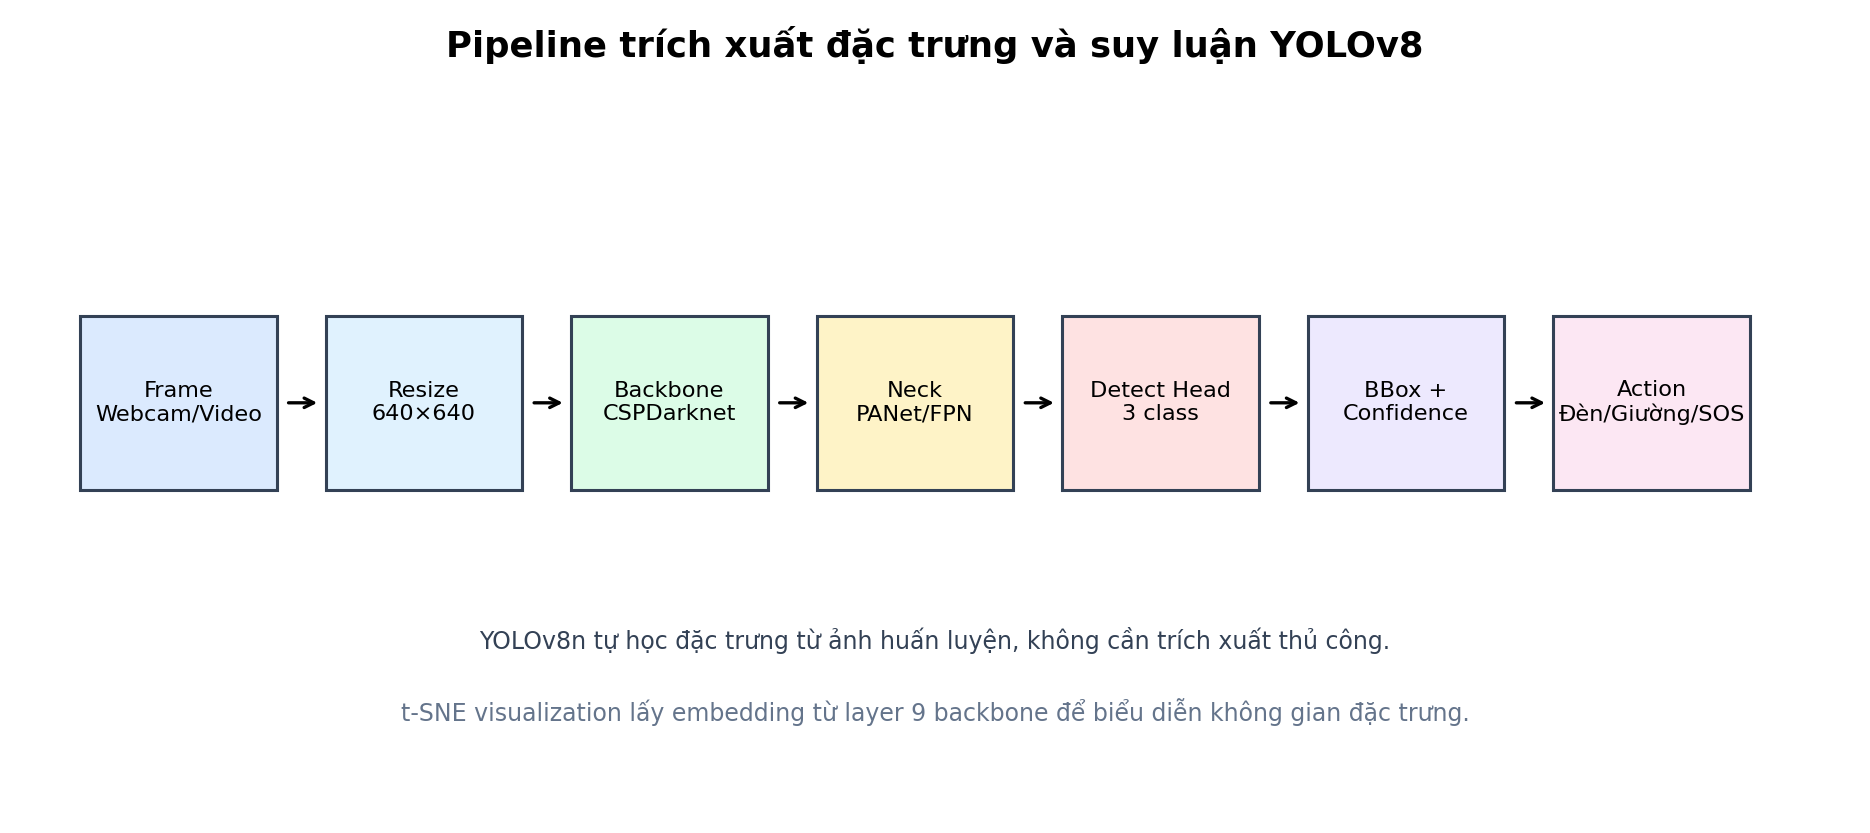
\includegraphics[width=\columnwidth]{figures/feature_extraction_pipeline.png}
\caption{Pipeline trích xuất đặc trưng.}
\end{figure}

\begin{table}[H]
\centering
\caption{\textbf{Bảng II.} Ánh xạ class YOLOv8n sang lệnh điều khiển thiết bị}
\label{tab:class_mapping}
\begin{tabular}{c|l|l|l}
\hline
\textbf{Class ID} & \textbf{Nhãn (Label)} & \textbf{Cử chỉ} & \textbf{Lệnh thiết bị} \\
\hline
0 & Nam\_Tay & Nắm tay & Bật/tắt đèn \\
1 & Chi\_Ngon\_Tro & Chỉ ngón trỏ & Nâng/hạ giường \\
2 & Xoe\_Tay & Xòe tay & SOS / Vuốt / Vẫy* \\
\hline
\end{tabular}
\end{table}

\textit{*Lớp Xoe\_Tay đóng vai trò kép: (1) Giữ tĩnh $\geq$5s → kích hoạt SOS; (2) Module MotionTracker phân tích quỹ đạo chuyển động ngang để phân biệt Vuốt trái/phải (swipe) và Vẫy tay (wave), không cần thêm class nhận dạng riêng.}

Đầu vào: ảnh RGB $640 \times 640$. Đầu ra: bounding box $(x, y, w, h)$, nhãn class cử chỉ và confidence score.

\subsection{Bộ lọc chống nhiễu và cơ chế Dwell-time}

Trong môi trường y tế, kích hoạt nhầm có thể gây hậu quả nghiêm trọng. Hệ thống thiết kế hai lớp bảo vệ:

\begin{figure}[h]
\centering
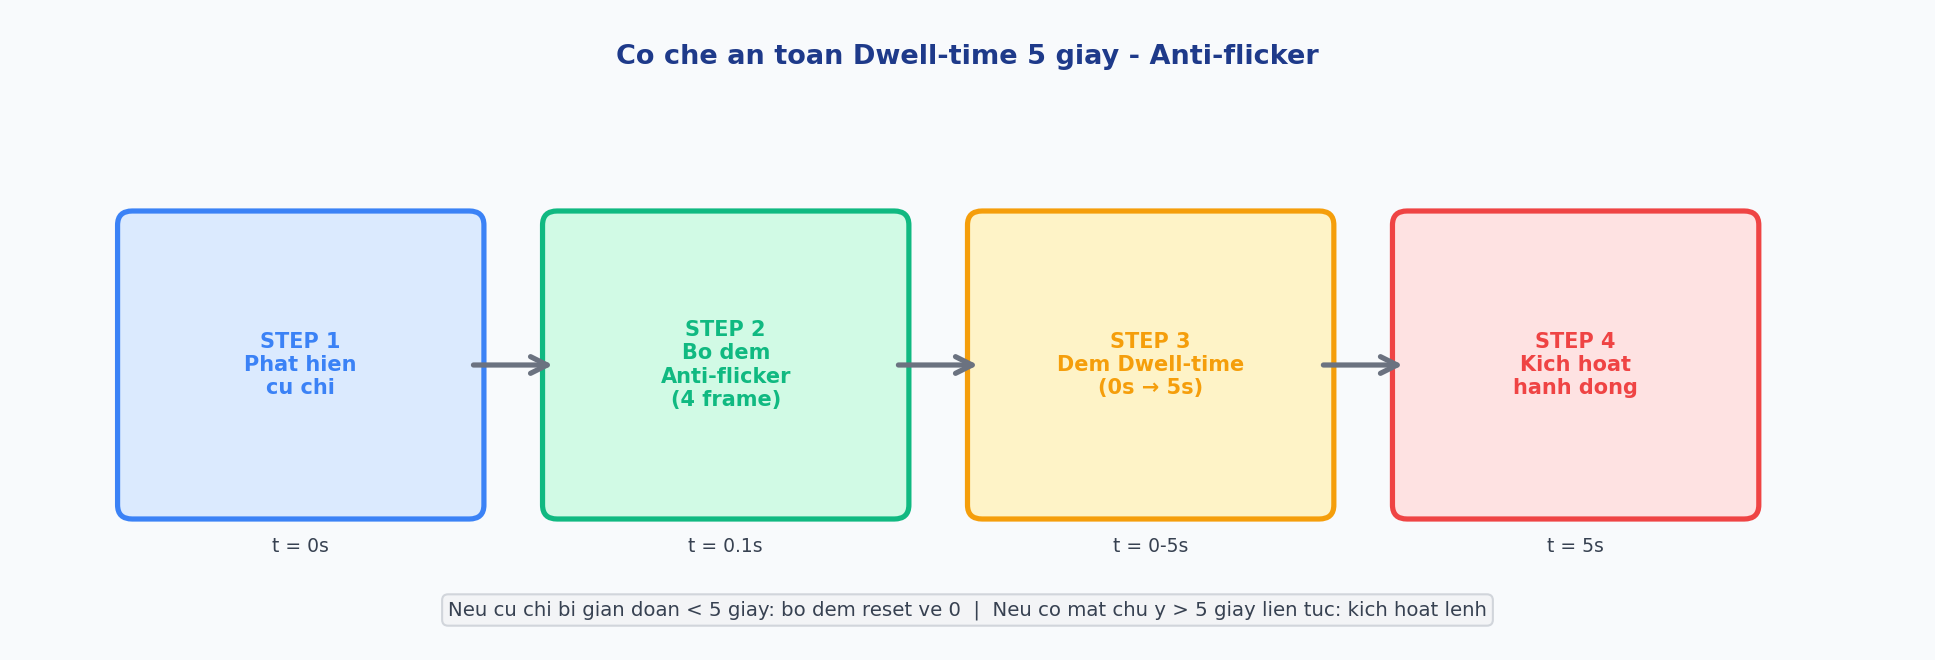
\includegraphics[width=\columnwidth]{figures/dwell_time_mechanism.png}
\caption{Cơ chế an toàn Dwell-time: Cử chỉ phải được giữ ổn định 5 giây trước khi kích hoạt hành động, đảm bảo bệnh nhân thực sự có chủ đích.}
\label{fig:dwell}
\end{figure}

\textbf{Lớp 1 --- Anti-flicker Buffer:} Sử dụng bộ đệm trượt $B$ frame. Cử chỉ chỉ được xác nhận khi xuất hiện ổn định $\geq M/B$ frame liên tiếp:
\begin{equation}
\text{stable}(t) = \begin{cases} g & \text{nếu } \text{count}(g, \text{buf}_B) \geq M \\ \text{stable}(t{-}1) & \text{ngược lại} \end{cases}
\end{equation}
với $B = 4$ (kích thước buffer), $M = 3$ (ngưỡng đa số).

\textbf{Lớp 2 --- Dwell-time 5 giây:} Bệnh nhân phải duy trì cử chỉ liên tục 5 giây:
\begin{equation}
\text{activate}(g) = \begin{cases} \text{true} & \text{nếu } t_{\text{hold}} \geq 5{,}0\text{s} \\ \text{false} & \text{ngược lại} \end{cases}
\end{equation}

\subsection{Nhận dạng cử chỉ động}

Bên cạnh cử chỉ tĩnh, hệ thống nhận dạng cử chỉ động thông qua module \texttt{MotionTracker} theo dõi quỹ đạo chuyển động ngang của bàn tay. Module này được kích hoạt khi YOLOv8n phát hiện và phân loại bàn tay vào class \textbf{Xoe\_Tay} (tay mở --- class phù hợp nhất cho cử chỉ vuốt/vẫy). Quỹ đạo tọa độ tâm bounding box theo trục $x$ được ghi lại liên tục và so sánh với các ngưỡng dịch chuyển:

\begin{itemize}[noitemsep]
    \item \textbf{Vuốt trái/phải:} Dịch chuyển ngang vượt ngưỡng $d > 0{,}16$ (theo tỉ lệ chiều rộng khung hình) trong cửa sổ 800ms với $\leq 1$ lần đổi chiều.
    \item \textbf{Vẫy tay:} Phát hiện $\geq 3$ lần đổi chiều ngang trong cửa sổ 1.400ms.
\end{itemize}

Cử chỉ động được kích hoạt \textbf{ngay lập tức} (không cần đợi 5s) vì bản thân chuyển động đã thể hiện rõ ý chí của người dùng. Trong thời gian \texttt{MotionTracker} đang theo dõi quỹ đạo, bộ đếm Dwell-time cho cử chỉ tĩnh bị tạm dừng để tránh nhận diện nhầm.

\subsection{Phản hồi giọng nói tiếng Việt}

Khi cử chỉ được kích hoạt, hệ thống phát giọng nói tiếng Việt thông qua \textbf{Web Speech API} (SpeechSynthesis):

\begin{table}[h]
\centering
\caption{Câu thoại phản hồi cho từng cử chỉ}
\label{tab:voice}
\begin{tabular}{l|l}
\hline
\textbf{Cử chỉ} & \textbf{Câu đọc tiếng Việt} \\
\hline
Nắm tay & ``Đã bật đèn phòng'' / ``Đã tắt đèn phòng'' \\
Chỉ ngón trỏ & ``Nâng đầu giường'' / ``Hạ đầu giường'' \\
Vuốt trái & ``Kéo rèm cửa vào'' \\
Vuốt phải & ``Mở rèm cửa ra'' \\
Xòe tay & ``Cảnh báo khẩn cấp! Đang gọi cứu trợ!'' \\
Vẫy tay & ``Đang gọi bác sĩ, vui lòng chờ'' \\
\hline
\end{tabular}
\end{table}

% ======================== 5. HUẤN LUYỆN ========================
\section{Huấn luyện mô hình}

\subsection{Pipeline huấn luyện}

\begin{figure}[h]
\centering
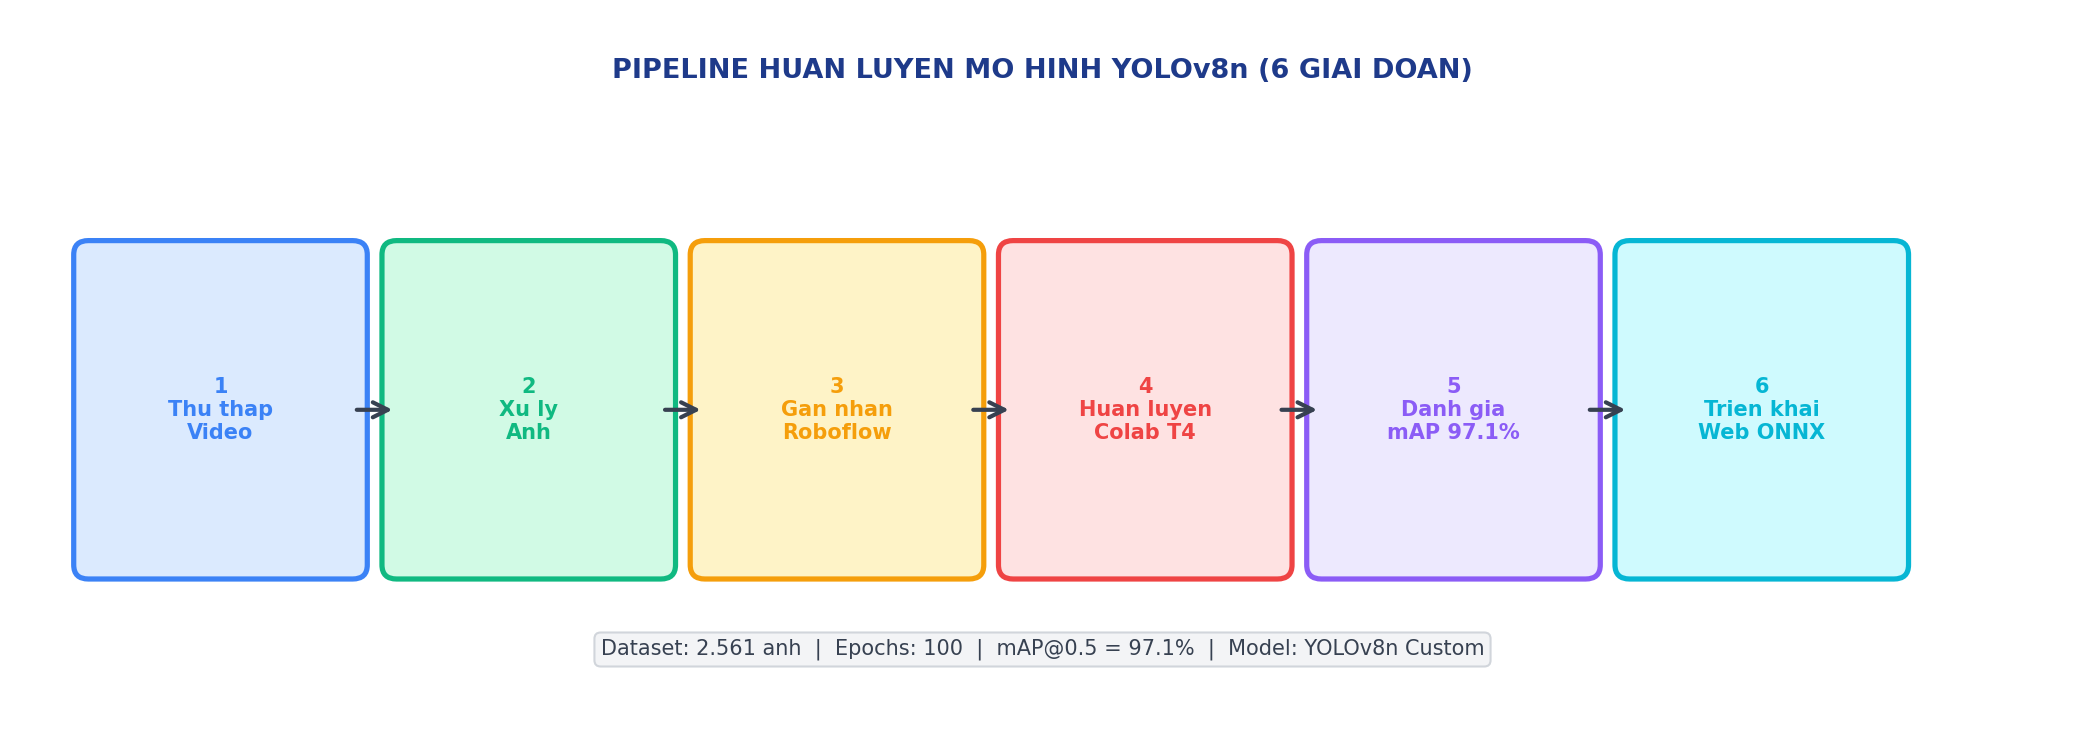
\includegraphics[width=\columnwidth]{figures/training_pipeline.png}
\caption{Pipeline hoàn chỉnh 6 giai đoạn từ thu thập video đến triển khai web.}
\label{fig:pipeline}
\end{figure}

\subsection{Siêu tham số}

Mô hình được huấn luyện trên Google Colab với GPU Tesla T4:

\begin{table}[h]
\centering
\caption{Siêu tham số huấn luyện}
\label{tab:hyperparams}
\begin{tabular}{l|c}
\hline
\textbf{Tham số} & \textbf{Giá trị} \\
\hline
Model gốc & yolov8n.pt \\
Số Epoch & 100 \\
Kích thước ảnh (imgsz) & 640 \\
Batch size & 16 \\
Thiết bị & GPU CUDA (Tesla T4) \\
Early Stopping (patience) & 20 \\
Optimizer & SGD + momentum \\
Learning rate & 0,01 \\
\hline
\end{tabular}
\end{table}

\begin{lstlisting}[float=htbp, caption={Lệnh huấn luyện YOLOv8 trên Colab}]
from ultralytics import YOLO

model = YOLO('yolov8n.pt')
results = model.train(
    data='data.yaml',
    epochs=100, imgsz=640,
    batch=16, device=0,
    patience=20,
    project='/content/runs',
    name='gesture_hospital_v1'
)
\end{lstlisting}

% ======================== 6. KẾT QUẢ ========================
\section{Độ chính xác và Kết quả thực nghiệm}

\subsection{Độ chính xác và Các chỉ số đánh giá}

Các chỉ số được đo lường trên tập thử nghiệm/val (proxy evaluation) khi thực hiện ánh xạ (map) mô hình sang cử chỉ.

\begin{figure}[H]
\centering

\includegraphics[width=\columnwidth]{figures/metrics_summary.png}
\caption{Tổng hợp các chỉ số đánh giá mô hình YOLOv8n (Custom). Mô hình đạt mAP@0.5 = \textbf{97,1\%}, được huấn luyện trong \textbf{100 epoch} trên Google Colab GPU Tesla T4.}
\end{figure}

\subsection{Ma trận nhầm lẫn}

Phân tích chi tiết sự nhầm lẫn giữa các lớp dự đoán và nhãn thực tế được thể hiện qua Ma trận nhầm lẫn (Confusion Matrix):

\begin{figure}[H]
\centering
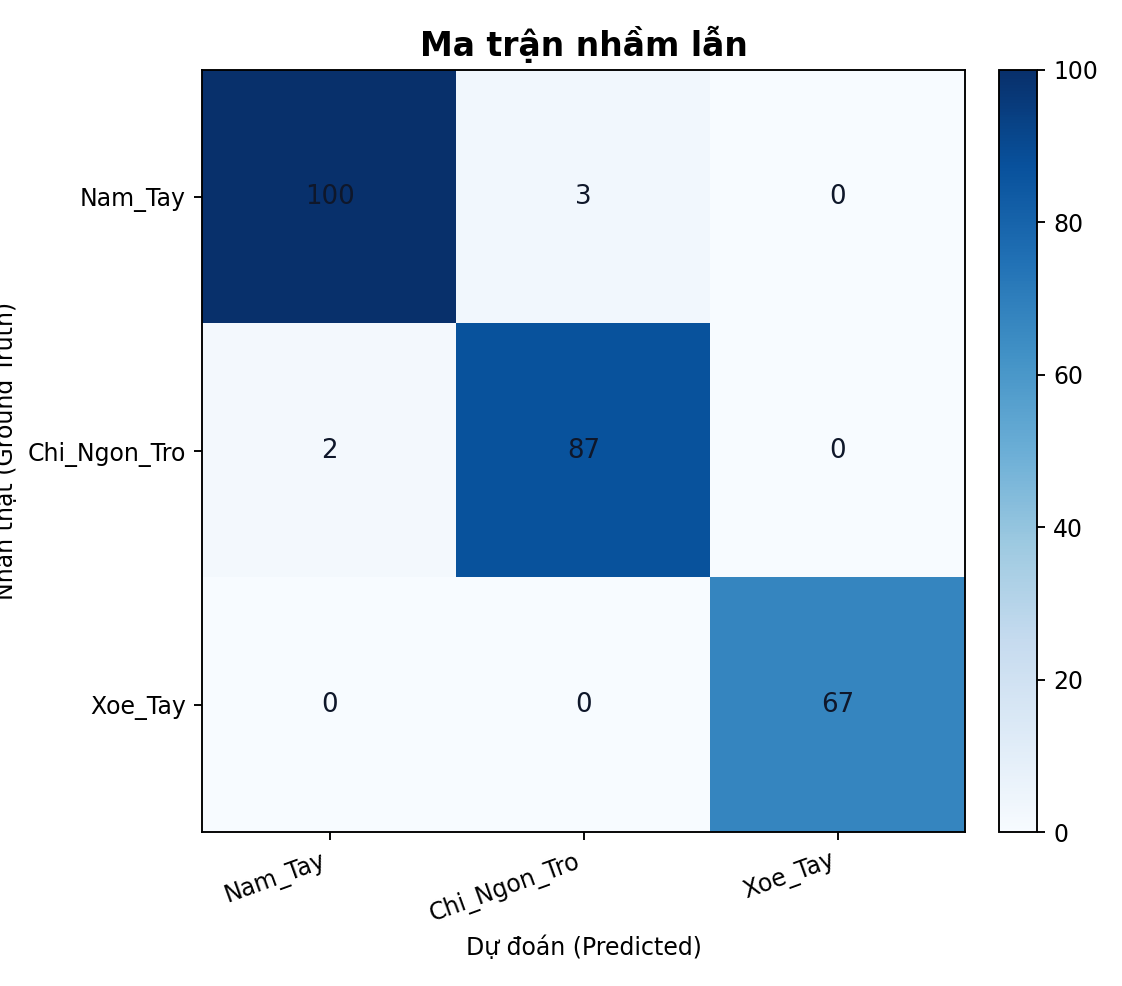
\includegraphics[width=\columnwidth]{figures/confusion_matrix_mapped.png}
\caption{Ma trận nhầm lẫn trên tập thử nghiệm.}
\end{figure}

\begin{figure}[H]
\centering
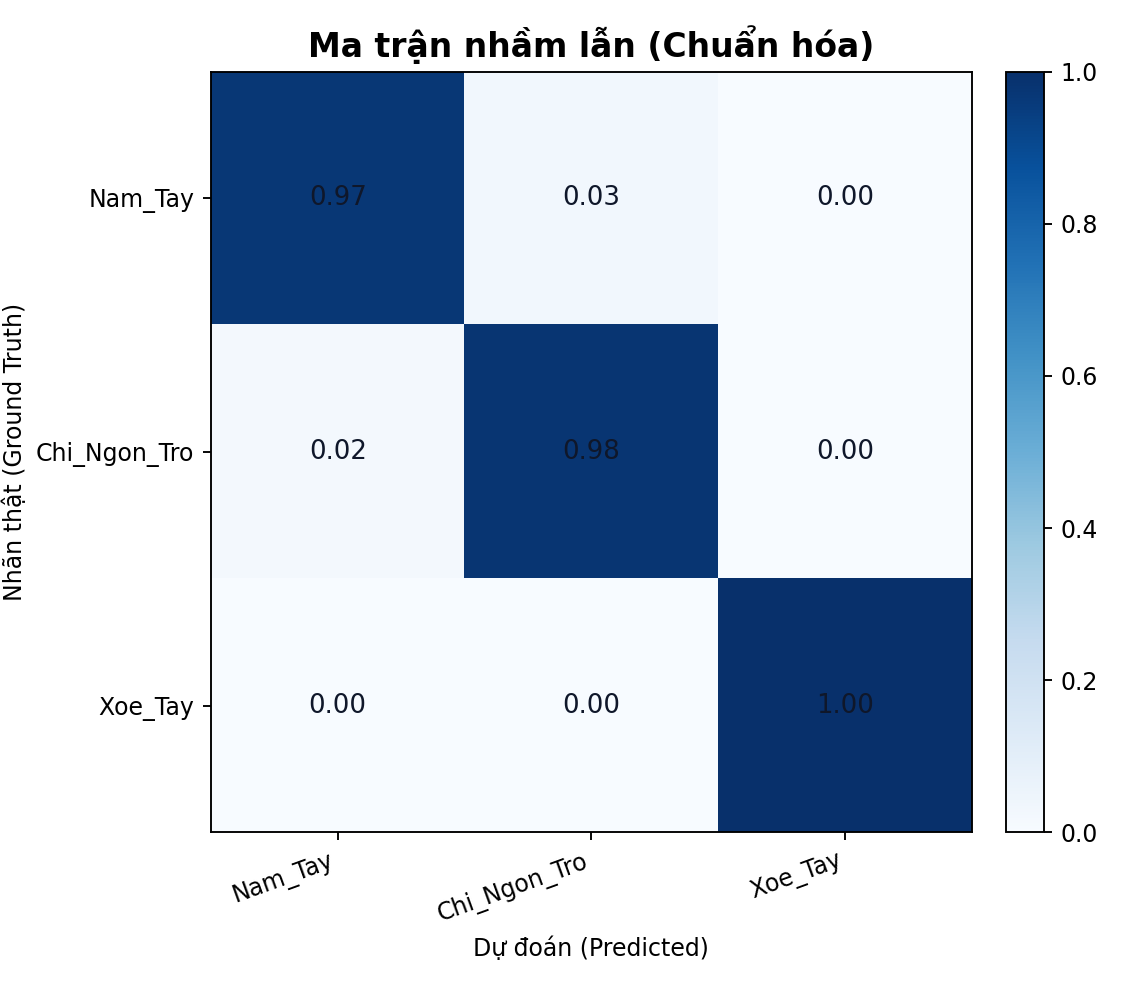
\includegraphics[width=\columnwidth]{figures/confusion_matrix_mapped_normalized.png}
\caption{Ma trận nhầm lẫn chuẩn hóa trên tập thử nghiệm.}
\end{figure}
\vspace{0.5cm}

\subsection{Phân tích không gian đặc trưng}

\begin{figure}[H]
\centering
\fbox{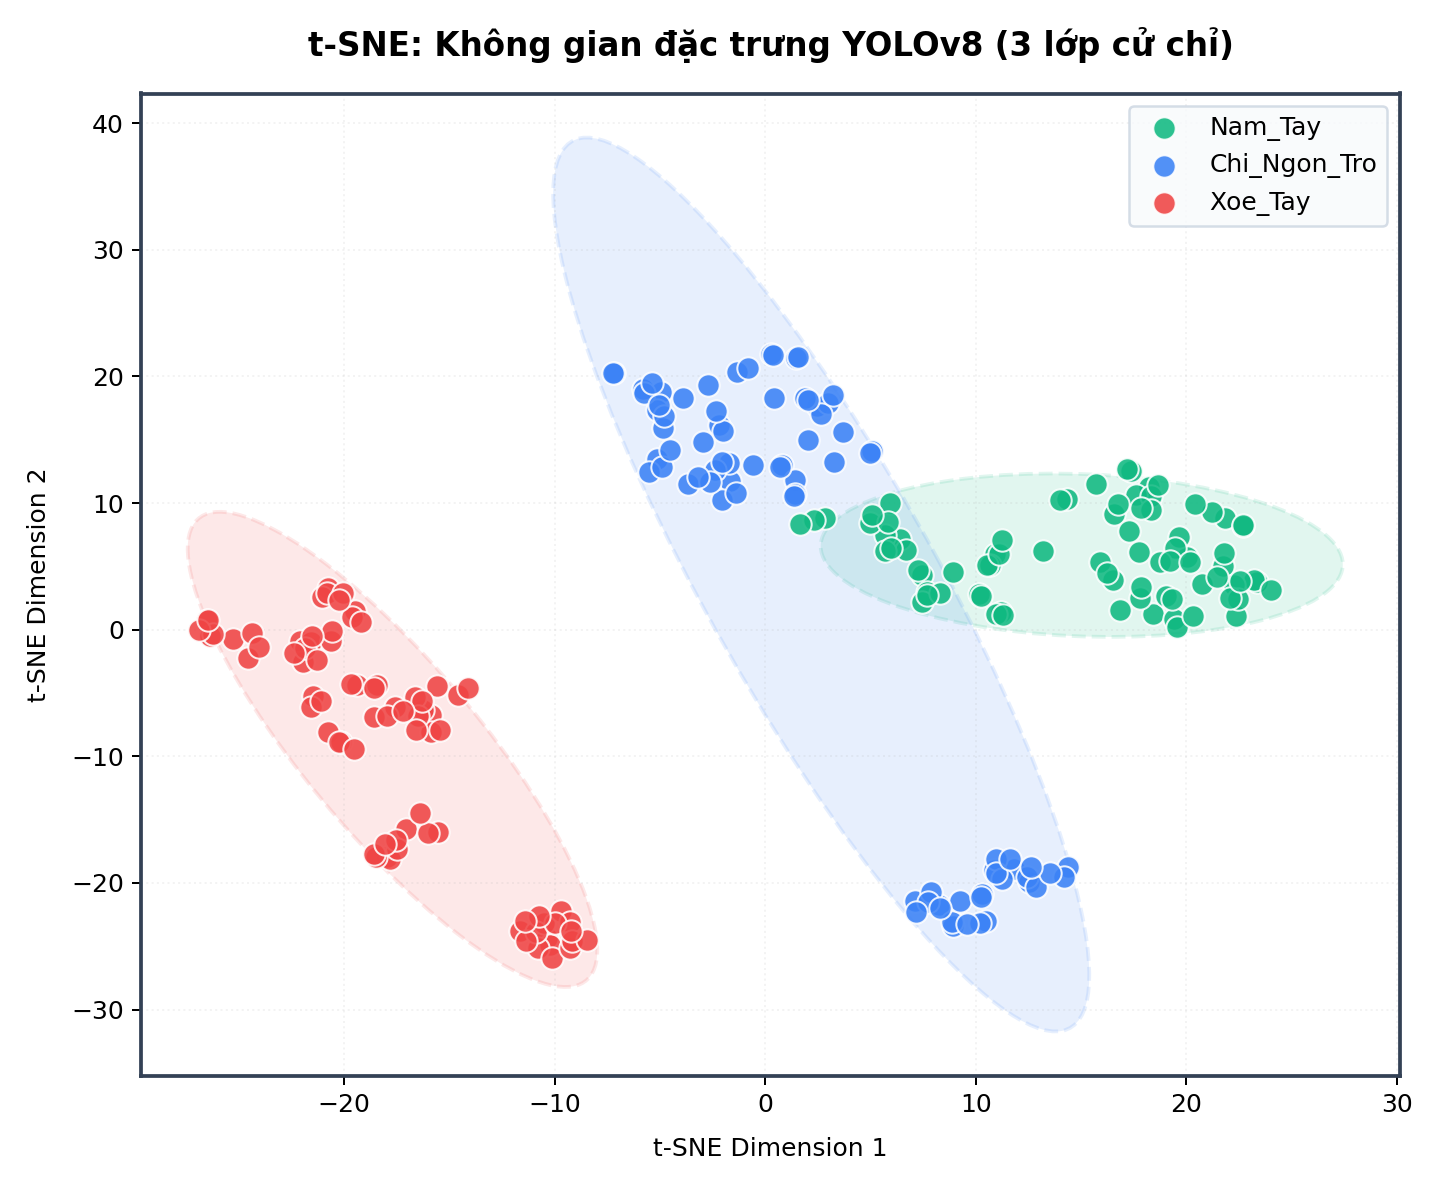
\includegraphics[width=0.95\columnwidth]{figures/tsne_features.png}}
\caption{t-SNE: Biểu diễn không gian đặc trưng trích xuất từ YOLOv8n (Custom). Các cụm màu phân tách rõ ràng cho thấy mô hình học được biểu diễn đặc trưng có tính phân biệt cao giữa các lớp cử chỉ.}
\end{figure}
\vspace{0.5cm}

% ======================== 7. GIAO DIỆN ========================
\section{Giao diện và triển khai}

\subsection{Dashboard điều khiển}

Giao diện web được xây dựng bằng HTML/CSS/JavaScript thuần, không phụ thuộc framework, hoạt động 100\% offline:

\begin{figure}[h]
\centering
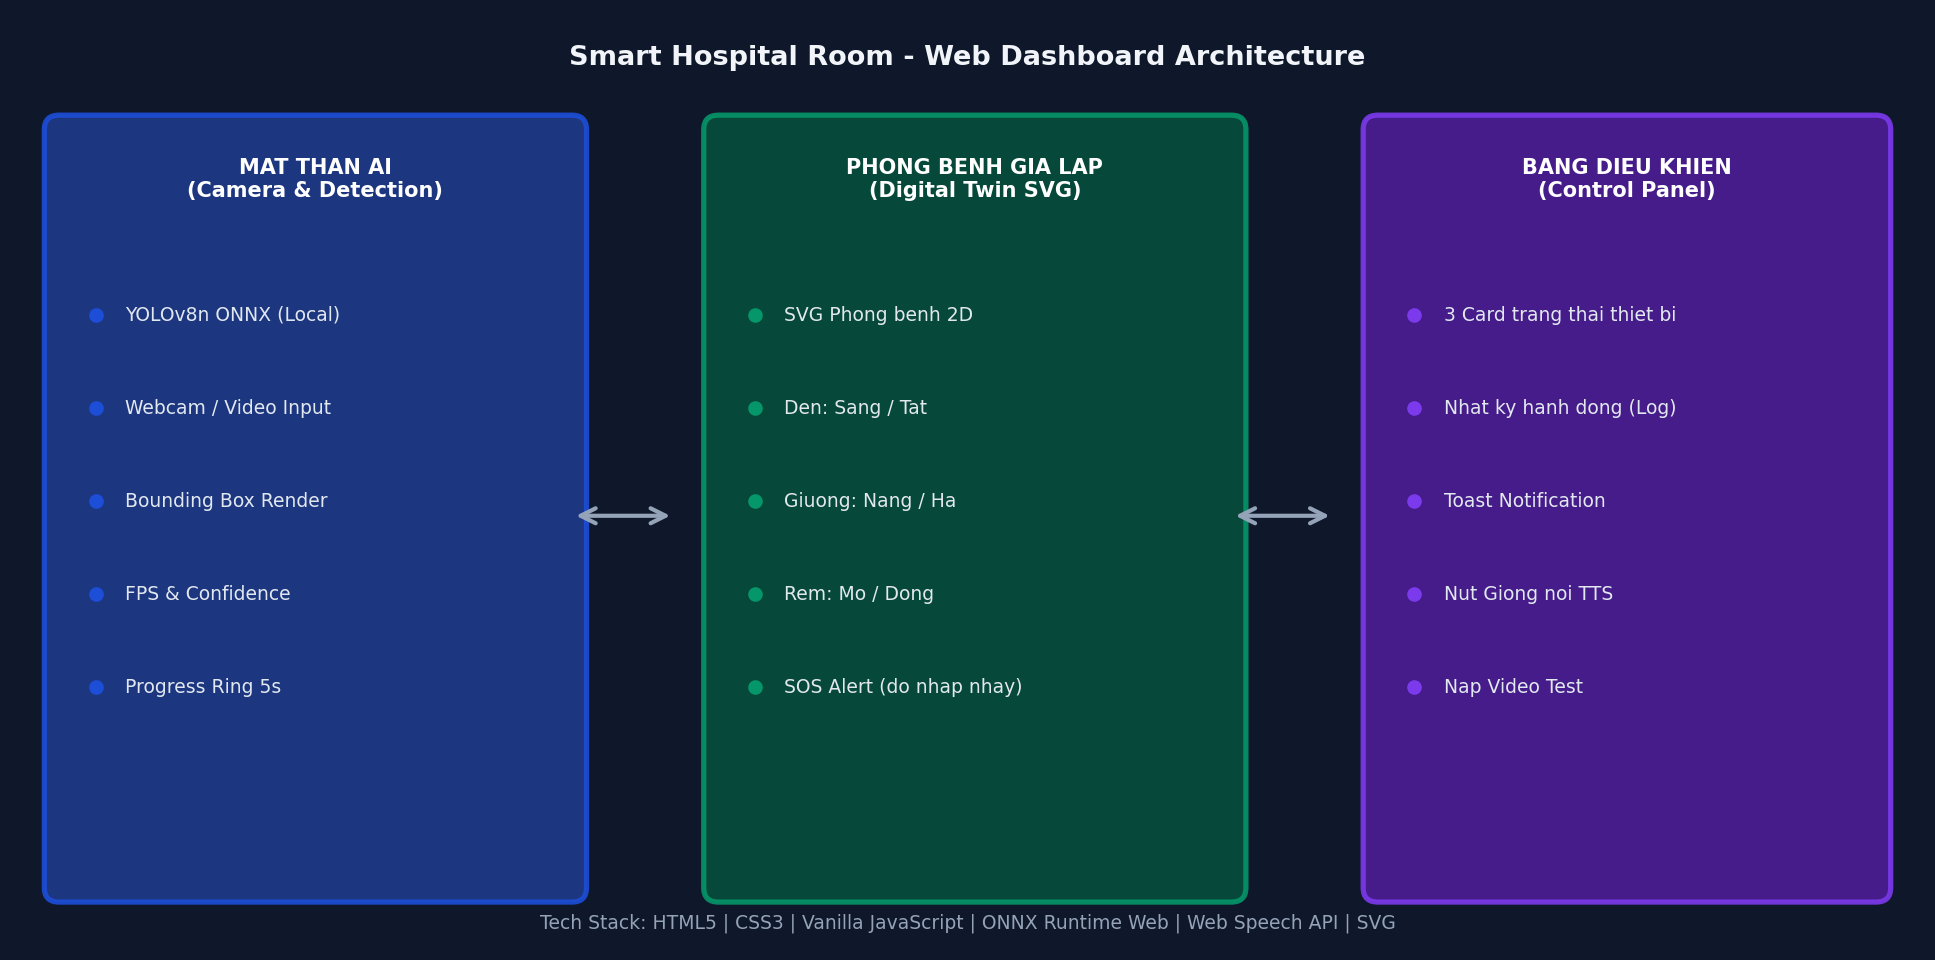
\includegraphics[width=\columnwidth]{figures/dashboard_ui.png}
\caption{Giao diện Dashboard y tế: Cột trái hiển thị camera AI với progress ring đếm giờ. Cột giữa mô phỏng phòng bệnh SVG. Cột phải hiển thị trạng thái thiết bị và nhật ký hành động.}
\label{fig:dashboard}
\end{figure}

\subsection{Các tính năng nổi bật}

\begin{itemize}[noitemsep]
    \item \textbf{Mắt Thần AI:} Hiển thị camera thời gian thực với bounding box nhận dạng, FPS, độ tin cậy.
    \item \textbf{Phòng Bệnh Giả Lập:} Mô hình SVG phòng bệnh phản ánh trạng thái thiết bị (đèn sáng/tối, giường nâng/hạ, rèm mở/đóng).
    \item \textbf{Progress Ring:} Vòng đếm ngược 5 giây trực quan, giúp bệnh nhân biết khi nào lệnh được kích hoạt.
    \item \textbf{Giọng nói TTS:} Phản hồi bằng tiếng Việt qua Web Speech API --- bật/tắt được qua nút giao diện.
    \item \textbf{Bảng Điều Khiển:} 3 card trạng thái thiết bị (Đèn/Giường/Rèm) cập nhật realtime + thông tin phòng bệnh.
    \item \textbf{Cảnh báo SOS:} Viền nhấp nháy đỏ bao toàn trang + giọng nói ``Cảnh báo khẩn cấp!''.
\end{itemize}

\subsection{Kiến trúc phần mềm}

Ứng dụng web gồm các module:

\begin{table}[h]
\centering
\caption{Cấu trúc module phần mềm}
\label{tab:modules}
\begin{tabular}{l|l}
\hline
\textbf{Module} & \textbf{Chức năng} \\
\hline
\texttt{app.js} & Bộ điều phối trung tâm, logic voice \\
\texttt{yolo-engine.js} & YOLOv8 ONNX inference \\
\texttt{digital-twin.js} & Điều khiển phòng bệnh SVG \\
\texttt{dashboard.js} & Widget UI, log, toast \\
\texttt{gestures.js} & MotionTracker cử chỉ động \\
\texttt{config.js} & Cấu hình tham số hệ thống \\
\hline
\end{tabular}
\end{table}

% ======================== 8. KẾT LUẬN ========================
\section{Kết luận và hướng phát triển}

\subsection{Kết quả đạt được}

Dự án đã xây dựng thành công hệ thống \textbf{Smart Hospital Room} --- điều khiển phòng bệnh bằng cử chỉ tay không tiếp xúc. Các kết quả nổi bật:

\begin{itemize}[noitemsep]
    \item Mô hình YOLOv8n (Custom) đạt mAP@0.5 = \textbf{97,1\%}; inference 41,7ms/frame trên CPU (tương đương $\sim$24 FPS), $>$30 FPS trên GPU.
    \item Nhận dạng 6 cử chỉ tay (3 tĩnh + 3 động) điều khiển 6 thiết bị/chức năng.
    \item Bộ lọc Dwell-time 5 giây đảm bảo an toàn, chống kích hoạt nhầm.
    \item Phản hồi giọng nói tiếng Việt thông qua Web Speech API.
    \item Giao diện Dashboard web hoạt động 100\% offline.
\end{itemize}

\subsection{Hạn chế}

\begin{itemize}[noitemsep]
    \item Bộ dữ liệu thu thập trong điều kiện phòng lab, chưa phản ánh đầy đủ biến thể phòng bệnh thực tế.
    \item Chưa có tập test độc lập ngoài tập validation.
    \item Cử chỉ động (vuốt, vẫy) dựa trên heuristic theo dõi chuyển động, chưa dùng mô hình học sâu.
\end{itemize}

\subsection{Hướng phát triển}

\begin{enumerate}[noitemsep]
    \item Tích hợp LSTM/Transformer nhận dạng chuỗi cử chỉ động phức tạp.
    \item Mở rộng thêm cử chỉ: gọi y tá, yêu cầu nước, điều khiển TV.
    \item Thu thập dữ liệu trong phòng bệnh thực tế.
    \item Triển khai trên thiết bị nhúng Jetson Nano hoặc Raspberry Pi.
    \item Tích hợp hướng dẫn sơ cứu lâm sàng trong chế độ SOS.
    \item Kết nối IoT thực tế: relay điều khiển đèn, motor giường bệnh.
\end{enumerate}

% ======================== TÀI LIỆU THAM KHẢO ========================
\begin{thebibliography}{00}

\bibitem{ref1} H.-G. Doan và cộng sự, ``A combination of user-guide scheme and kernel descriptor on rgb-d data for robust and realtime hand posture recognition,'' \textit{Engineering Applications of Artificial Intelligence}, vol. 49, tr. 103--113, 2016.

\bibitem{ref2} J. Redmon, S. Divvala, R. Girshick, và A. Farhadi, ``You only look once: Unified, real-time object detection,'' trong \textit{Proc. IEEE/CVF CVPR}, 2016, tr. 779--788.

\bibitem{ref4} T.-H. Le, T.-H. Tran, và C. Pham, ``The internet-of-things based hand gestures using wearable sensors for human machine interaction,'' trong \textit{2019 International Conference on MAPR}, IEEE, 2019, tr. 1--6.

\bibitem{ref5} A. Dosovitskiy và cộng sự, ``An Image is Worth 16$\times$16 Words,'' trong \textit{Proc. ICLR}, 2021.

\bibitem{ref7} G. Jocher, A. Chaurasia, và J. Qiu, ``Ultralytics YOLOv8,'' 2023. [Online]. Available: \url{https://github.com/ultralytics/ultralytics}

\bibitem{ref9} K. He, X. Zhang, S. Ren, và J. Sun, ``Deep Residual Learning for Image Recognition,'' trong \textit{Proc. IEEE/CVF CVPR}, tr. 770--778, 2016.

\bibitem{ref10} J. Redmon và A. Farhadi, ``YOLOv3: An incremental improvement,'' \textit{arXiv:1804.02767}, 2018.

\bibitem{ref11} A. Bochkovskiy, C. Wang, và H. M. Liao, ``YOLOv4: Optimal speed and accuracy of object detection,'' \textit{CoRR}, vol. abs/2004.10934, 2020.

\bibitem{ref12} A. Paszke và cộng sự, ``PyTorch: An Imperative Style, High-Performance Deep Learning Library,'' trong \textit{NeurIPS}, 2019.

\bibitem{ref13} L. van der Maaten và G. Hinton, ``Visualizing Data using t-SNE,'' \textit{JMLR}, tập 9, số 11, 2008.

\end{thebibliography}

\end{document}
